\documentclass[11pt,a4paper]{article}

% Packages
\usepackage[utf8]{inputenc}
\usepackage[T1]{fontenc}
\usepackage{geometry}
\geometry{top=2.5cm, bottom=3cm, left=2.5cm, right=2.5cm, headheight=14pt}
\usepackage{float}
\usepackage{fancyhdr}
\usepackage{tikz}
\usetikzlibrary{positioning, arrows.meta, shapes, calc, fit, backgrounds}
\usepackage{pgfplots}
\pgfplotsset{compat=1.18}
\usepackage{listings}
\usepackage{xcolor}
\usepackage{amsmath}
\usepackage{hyperref}

% Code Listing Style
\definecolor{codegreen}{rgb}{0,0.6,0}
\definecolor{codegray}{rgb}{0.5,0.5,0.5}
\definecolor{codepurple}{rgb}{0.58,0,0.82}
\definecolor{backcolour}{rgb}{0.95,0.95,0.92}
\lstdefinestyle{mystyle}{
    backgroundcolor=\color{backcolour},   
    commentstyle=\color{codegreen},
    keywordstyle=\color{magenta},
    numberstyle=\tiny\color{codegray},
    stringstyle=\color{codepurple},
    basicstyle=\ttfamily\footnotesize,
    breakatwhitespace=false,         
    breaklines=true,                 
    captionpos=b,                    
    keepspaces=true,                 
    numbers=left,                    
    numbersep=5pt,                  
    showspaces=false,                
    showstringspaces=false,
    showtabs=false,                  
    tabsize=2
}
\lstset{style=mystyle}

% Header and Footer Configuration
\pagestyle{fancy}
\fancyhf{} % Clear all header and footer fields
\fancyhead[C]{\thepage} % Page number centered on top
\fancyfoot[C]{UM5IN160 - PACC \textbar{} Lab 2 - Single-core CPU Optimizations \textbar{} Wilson Genevieve}
\renewcommand{\headrulewidth}{0pt} % Remove header line if desired, or keep with 0.4pt
\renewcommand{\footrulewidth}{0.4pt} % Add footer line

% Document Info
\title{\vspace{-1.5cm}\textbf{UM5IN160 - PACC}\\Lab 2: Single-core CPU Optimizations\\Revision Report}
\author{Wilson Genevieve}
\date{November 2026}

\begin{document}

\maketitle
\thispagestyle{fancy} % Ensure the first page has the correct footer/header

\begin{abstract}
This report details the step-by-step optimization of a 2D image blurring kernel (stencil algorithm) executed on the Dalek cluster (az4-n4090-0 / az4-mixed partition). The goal is to explore how manual single-core CPU optimizations---such as loop unrolling, function inlining, memory rotation, and algorithmic reduction---can drastically improve execution time compared to naive compiler optimizations.
\end{abstract}

\section{Introduction and Baseline Testing}
The \texttt{blur} kernel applies a convolution matrix to blur an image. By default, EasyPAP compiles with the \texttt{-O2} optimization flag. To isolate the effects of our manual C-code optimizations, we must first disable the compiler's automatic optimizations by compiling with \texttt{-O0}.

\subsection{Basic Testing and \texttt{-O0} Compilation}
With default CMake flags (\texttt{-O2} or \texttt{-O3}), the baseline execution time was \textbf{1246.842 ms}.
Recompiling with \texttt{-O0} allows us to observe the true cost of unoptimized memory accesses and loop overheads:
\begin{lstlisting}[language=bash]
cmake -S . -B build -DCMAKE_C_FLAGS_RELEASE="-O0" -DCMAKE_CXX_FLAGS_RELEASE="-O0"
cmake --build build --parallel
./run -n -k blur --load-image images/1024.png -i 100 -v seq -wt default
\end{lstlisting}
The baseline unoptimized execution time soared to \textbf{5433.210 ms}. This establishes our starting metric.

\section{Step-by-Step Optimizations}

\subsection{Optimization 0: No Border (\texttt{default\_nb})}
To simplify our fast inner loops, we first removed the border management logic.

\textbf{Before (Original with bounds checking):}
\begin{lstlisting}[language=C]
for (int i = y; i < y + height; i++) {
    for (int j = x; j < x + width; j++) {
        int i_d = (i > 0) ? i - 1 : i;
        // ... bounds checking ...
    }
}
\end{lstlisting}

\textbf{After (Optimized without borders):}
\begin{lstlisting}[language=C]
// Simplified boundary loops: start at +1, end at -1
for (int i = y + 1; i < y + height - 1; i++) {
    for (int j = x + 1; j < x + width - 1; j++) {
        // ... nested loops without any 'if' boundary checks ...
    }
}
\end{lstlisting}

\begin{itemize}
    \item \textbf{Result:} 5354.464 ms
    \item \textbf{Analysis:} The negligible speedup confirms that the border pixels constitute a tiny fraction of the total computational workload ($O(N)$ vs $O(N^2)$ for the center). However, this simplification paves the way for aggressive inner-loop unrolling.
\end{itemize}

\subsection{Optimization 1: Loop Unrolling on X-axis (\texttt{optim1})}
Loop unrolling removes the overhead of loop counter increments and condition checking. In this step, the inner \texttt{xloc} loop was manually expanded to explicitly calculate the three horizontal neighboring pixels.

\textbf{Before (Nested loops):}
\begin{lstlisting}[language=C]
for (int yloc = i - 1; yloc <= i + 1; yloc++) {
    for (int xloc = j - 1; xloc <= j + 1; xloc++) {
        unsigned c = cur_img(yloc, xloc);
        r += ezv_c2r(c); // ... plus g, b, a
    }
}
\end{lstlisting}

\textbf{After (X-axis unrolled):}
\begin{lstlisting}[language=C]
// Inner xloc loop removed, manual extraction for j-1, j, j+1
for (int yloc = i - 1; yloc <= i + 1; yloc++) {
    unsigned c1 = cur_img(yloc, j - 1);
    r += ezv_c2r(c1); g += ezv_c2g(c1); b += ezv_c2b(c1); a += ezv_c2a(c1);
    
    unsigned c2 = cur_img(yloc, j);
    r += ezv_c2r(c2); g += ezv_c2g(c2); b += ezv_c2b(c2); a += ezv_c2a(c2);
    
    unsigned c3 = cur_img(yloc, j + 1);
    r += ezv_c2r(c3); g += ezv_c2g(c3); b += ezv_c2b(c3); a += ezv_c2a(c3);
}
\end{lstlisting}

\begin{itemize}
    \item \textbf{Result:} 5114.760 ms
    \item \textbf{Analysis:} A modest gain of $\sim$240 ms. The CPU is spared the branch prediction and counter management for the innermost loop.
\end{itemize}

\begin{figure}[H]
\centering
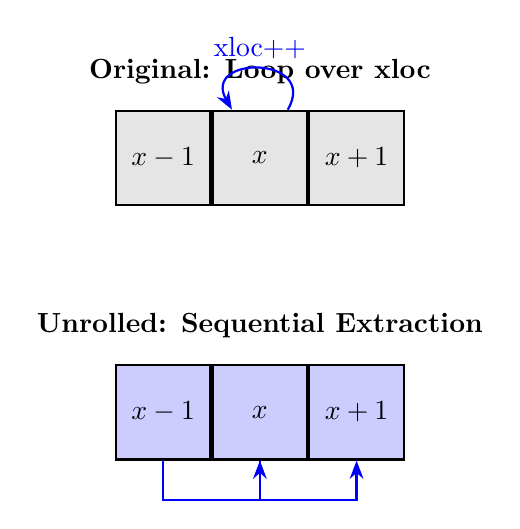
\begin{tikzpicture}[
    cell/.style={rectangle, draw=black, thick, minimum size=1.2cm, align=center, font=\sffamily},
    arrow/.style={-Stealth, thick, blue}
]
    % Loop representation
    \node (l1) [cell, fill=gray!20] {$x-1$};
    \node (l2) [cell, right=0cm of l1, fill=gray!20] {$x$};
    \node (l3) [cell, right=0cm of l2, fill=gray!20] {$x+1$};
    
    \node[above=0.2cm of l2, font=\bfseries] {Original: Loop over xloc};
    \draw[arrow, loop above, distance=0.8cm, out=60, in=120] (l2) to node[above] {xloc++} (l2);

    % Unrolled representation
    \node (u1) [cell, fill=blue!20, below=2cm of l1] {$x-1$};
    \node (u2) [cell, right=0cm of u1, fill=blue!20] {$x$};
    \node (u3) [cell, right=0cm of u2, fill=blue!20] {$x+1$};

    \node[above=0.2cm of u2, font=\bfseries] {Unrolled: Sequential Extraction};
    \draw[arrow] (u1.south) -- +(0,-0.5) -| (u2.south);
    \draw[arrow] (u2.south) -- +(0,-0.5) -| (u3.south);

\end{tikzpicture}
\caption{Visual representation of removing the iterative overhead via X-axis Loop Unrolling.}
\end{figure}

\subsection{Optimization 2: Loop Unrolling on Y-axis (\texttt{optim2})}
We extended the unrolling to the Y-axis, completely eliminating the $3\times3$ nested loops.

\textbf{Before (Y-axis loop remaining):}
\begin{lstlisting}[language=C]
for (int yloc = i - 1; yloc <= i + 1; yloc++) {
    unsigned c1 = cur_img(yloc, j - 1);
    // ... color extractions ...
}
\end{lstlisting}

\textbf{After (Both axes unrolled):}
\begin{lstlisting}[language=C]
// Both xloc and yloc loops removed. 9 explicit pixel fetches:
unsigned c1 = cur_img(i - 1, j - 1);
r += ezv_c2r(c1); g += ezv_c2g(c1); b += ezv_c2b(c1); a += ezv_c2a(c1);
// ... (Repeated sequentially for c2 through c9) ...
unsigned c9 = cur_img(i + 1, j + 1);
r += ezv_c2r(c9); g += ezv_c2g(c9); b += ezv_c2b(c9); a += ezv_c2a(c9);
\end{lstlisting}

\begin{itemize}
    \item \textbf{Result:} 5182.366 ms (Time Increased!)
    \item \textbf{Analysis:} Unrolling the Y-axis unexpectedly worsened performance. While we removed the loop counters, we explicitly wrote out 9 pixel fetches. Under \texttt{-O0}, each pixel requires 4 color extractions (\texttt{ezv\_c2r}, etc.) and 1 pack function (\texttt{ezv\_rgba}). This resulted in \textbf{37 discrete function calls per pixel}. The massive overhead of context switching and memory jumping for these function calls completely negated the unrolling benefits.
\end{itemize}

\begin{figure}[H]
\centering
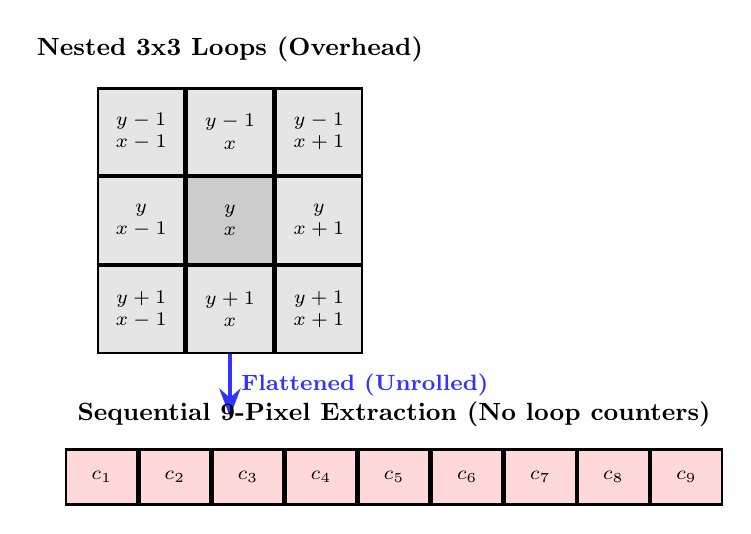
\begin{tikzpicture}[
    cell/.style={rectangle, draw=black, thick, minimum size=1.1cm, align=center, font=\sffamily\scriptsize},
    seq/.style={rectangle, draw=black, fill=red!15, thick, minimum width=0.9cm, minimum height=0.7cm, font=\sffamily\scriptsize}
]
    % 3x3 Grid
    \node (g1) [cell, fill=gray!20] {$y-1$\\$x-1$};
    \node (g2) [cell, right=0cm of g1, fill=gray!20] {$y-1$\\$x$};
    \node (g3) [cell, right=0cm of g2, fill=gray!20] {$y-1$\\$x+1$};
    \node (g4) [cell, below=0cm of g1, fill=gray!20] {$y$\\$x-1$};
    \node (g5) [cell, right=0cm of g4, fill=gray!40] {$y$\\$x$};
    \node (g6) [cell, right=0cm of g5, fill=gray!20] {$y$\\$x+1$};
    \node (g7) [cell, below=0cm of g4, fill=gray!20] {$y+1$\\$x-1$};
    \node (g8) [cell, right=0cm of g7, fill=gray!20] {$y+1$\\$x$};
    \node (g9) [cell, right=0cm of g8, fill=gray!20] {$y+1$\\$x+1$};
    
    \node[above=0.2cm of g2, font=\bfseries\small] {Nested 3x3 Loops (Overhead)};
    
    % Down Arrow
    \draw[-Stealth, ultra thick, blue!80] (g8.south) -- +(0,-0.8) node[midway, right, font=\bfseries\footnotesize] {Flattened (Unrolled)};
    
    % Sequence
    \node (s1) [seq, below=1.2cm of g7, xshift=-0.5cm] {$c_1$};
    \node (s2) [seq, right=0cm of s1] {$c_2$};
    \node (s3) [seq, right=0cm of s2] {$c_3$};
    \node (s4) [seq, right=0cm of s3] {$c_4$};
    \node (s5) [seq, right=0cm of s4] {$c_5$};
    \node (s6) [seq, right=0cm of s5] {$c_6$};
    \node (s7) [seq, right=0cm of s6] {$c_7$};
    \node (s8) [seq, right=0cm of s7] {$c_8$};
    \node (s9) [seq, right=0cm of s8] {$c_9$};

    \node[above=0.15cm of s5, font=\bfseries\small] {Sequential 9-Pixel Extraction (No loop counters)};
\end{tikzpicture}
\caption{Y-axis loop unrolling completely flattens the 2D memory access pattern into a linear sequence of instructions.}
\end{figure}


\subsection{Optimization 3: Inline Function Calls (\texttt{optim3})}
To resolve the function call overhead discovered in \texttt{optim2}, we manually inlined the color extraction functions, replacing them with raw bitwise operations directly within the loop (e.g., \texttt{(uint8\_t)(c >> 8)}).

\textbf{Before (Function calls):}
\begin{lstlisting}[language=C]
unsigned c1 = cur_img(i - 1, j - 1);
r += ezv_c2r(c1); g += ezv_c2g(c1); b += ezv_c2b(c1); a += ezv_c2a(c1);
// ...
next_img(i, j) = ezv_rgba(r, g, b, a);
\end{lstlisting}

\textbf{After (Manual inlining):}
\begin{lstlisting}[language=C]
// Manual bitwise shifting replaces ezv_* function jumps per pixel
unsigned c1 = cur_img(i - 1, j - 1);
r += (uint8_t)c1; 
g += (uint8_t)(c1 >> 8); 
b += (uint8_t)(c1 >> 16); 
a += (uint8_t)(c1 >> 24);

// ... at the end of the loop, pack pixel manually
next_img(i, j) = r | (g << 8) | (b << 16) | (a << 24);
\end{lstlisting}

\begin{itemize}
    \item \textbf{Result:} 2733.973 ms
    \item \textbf{Analysis:} The execution time was nearly cut in half. This drastically highlights the hardware cost of function calls (stack pushes/pops and instruction pointer jumps) when compiler inlining (\texttt{-O3}) is disabled.
\end{itemize}

\subsection{Optimization 4: Variables Rotation (\texttt{optim4})}
This optimization addresses the "Memory Wall." In a sliding $3\times3$ stencil, 6 of the 9 pixels needed for column $j+1$ were already fetched from Main Memory for column $j$. By saving the vertical column totals and passing them horizontally, we eliminate redundant RAM accesses.

\textbf{Before (9 independent loads per pixel):}
\begin{lstlisting}[language=C]
// 9 explicit cur_img calls inside the j loop
unsigned c1 = cur_img(i - 1, j - 1);
// ...
unsigned c9 = cur_img(i + 1, j + 1);
\end{lstlisting}

\textbf{After (Variables rotation):}
\begin{lstlisting}[language=C]
// 1. Fetch ONLY the brand new Right column from RAM
unsigned c3 = cur_img(i - 1, j + 1); 
// ... extract and add to r_right, g_right, etc.

// 2. Add the reduced columns together using fast CPU registers
unsigned r = r_left + r_center + r_right; 
// ... (averaging logic)

// 3. Shift the "conveyor belt" (Registers) for the next pixel
r_left = r_center;
r_center = r_right;
\end{lstlisting}

\begin{itemize}
    \item \textbf{Result:} 1449.473 ms
    \item \textbf{Analysis:} A massive performance leap. Reducing memory reads from 9 pixels down to 3 pixels per iteration maximizes cache efficiency and keeps the CPU ALUs fed with data.
\end{itemize}

\begin{figure}[H]
\centering
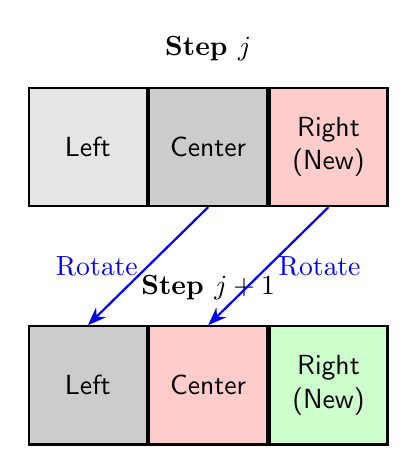
\begin{tikzpicture}[
    cell/.style={rectangle, draw=black, thick, minimum size=1.5cm, align=center, font=\sffamily},
    arrow/.style={-Stealth, thick, blue}
]
    % Old diagram for variables rotation (Simpler 3x3 sliding view)
    \node (p1) [cell, fill=gray!20] {Left};
    \node (p2) [cell, right=0cm of p1, fill=gray!40] {Center};
    \node (p3) [cell, right=0cm of p2, fill=red!20] {Right\\(New)};

    \node[above=0.2cm of p2, font=\bfseries] {Step $j$};
    
    \node (n1) [cell, fill=gray!40, below=1.5cm of p1] {Left};
    \node (n2) [cell, right=0cm of n1, fill=red!20] {Center};
    \node (n3) [cell, right=0cm of n2, fill=green!20] {Right\\(New)};

    \node[above=0.2cm of n2, font=\bfseries] {Step $j+1$};

    \draw[arrow] (p2.south) -- (n1.north) node[midway, left] {Rotate};
    \draw[arrow] (p3.south) -- (n2.north) node[midway, right] {Rotate};

\end{tikzpicture}
\caption{Variables Rotation Concept. As the stencil moves from $j$ to $j+1$, the old Center becomes the new Left, and the old Right becomes the new Center. Only the new Right column is fetched from memory.}
\end{figure}

\subsection{Optimization 5 \& 6: Manage Borders and Reduction}

\textbf{Before (No borders managed):}
\begin{lstlisting}[language=C]
// fast loop only processes the center, leaving edges uncomputed
for (int i = y + 1; i < y + height - 1; i++) {
    // ...
}
\end{lstlisting}

\textbf{After (Border pass added via \texttt{continue}):}
\begin{lstlisting}[language=C]
// optim5: Separate pass just for the edges
for (int i = y; i < y + height; i++) {
    for (int j = x; j < x + width; j++) {
        // Skip the already-processed center grid!
        if (i > y && i < y + height - 1 && j > x && j < x + width - 1) {
            continue; 
        }
        // ... original safe border computation logic ...
    }
}
\end{lstlisting}

\begin{itemize}
    \item \textbf{\texttt{optim5} (Manage Borders):} 1584.361 ms. We re-introduced border calculations using a second pass with a \texttt{continue} statement for the center grid. The slight time increase is due to evaluating the \texttt{if} condition 1,000,000 times.
    \item \textbf{\texttt{optim6} (Reduction):} Already successfully implemented during \texttt{optim4}. We pre-summed the 3 vertical pixels per column \textit{before} rotation. 
\end{itemize}

\textbf{Before (No Reduction):}
\begin{lstlisting}[language=C]
// 9 separate pixel additions every iteration
r += c1_r + c2_r + c3_r + c4_r + c5_r + c6_r + c7_r + c8_r + c9_r;
\end{lstlisting}

\textbf{After (With Reduction):}
\begin{lstlisting}[language=C]
// optim6 (Reduction): 3 vertical pixels summed into 1 variable first
unsigned r_left = 0;
unsigned c1 = cur_img(i - 1, x); r_left += (uint8_t)c1; 
unsigned c4 = cur_img(i, x);     r_left += (uint8_t)c4; 
unsigned c7 = cur_img(i + 1, x); r_left += (uint8_t)c7; 
\end{lstlisting}

This $3 \rightarrow 1$ reduction means we only added 3 variables for the final average instead of 9, heavily optimizing ALU usage.

\section{Compiler Optimizations Comparison (\texttt{-O3})}
To conclude, we re-enabled the compiler's maximum optimization flags (\texttt{-O3}) to test if our hand-written architectural changes could out-perform the compiler's best automatic attempts on the default code.

\begin{lstlisting}[language=bash]
cmake -S . -B build -DCMAKE_C_FLAGS_RELEASE="-O3" -DCMAKE_CXX_FLAGS_RELEASE="-O3"
cmake --build build --parallel
\end{lstlisting}

\begin{itemize}
    \item \textbf{\texttt{default} with \texttt{-O3}:} 1249.174 ms
    \item \textbf{\texttt{optim4/6} with \texttt{-O3}:} 461.541 ms
\end{itemize}

\begin{figure}[H]
\centering
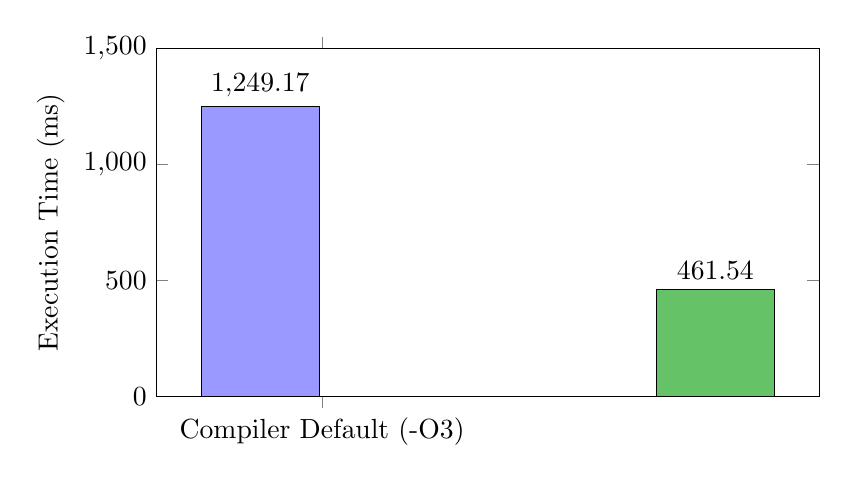
\begin{tikzpicture}
\begin{axis}[
    ybar,
    bar width=1.5cm,
    enlarge x limits=0.5,
    legend style={at={(0.5,-0.2)}, anchor=north, legend columns=-1},
    ylabel={Execution Time (ms)},
    symbolic x coords={Compiler Default (-O3), Hand-Optimized (-O3)},
    xtick=data,
    nodes near coords,
    nodes near coords align={vertical},
    ymin=0, ymax=1500,
    width=10cm,
    height=6cm
]
\addplot[fill=blue!40] coordinates {(Compiler Default (-O3),1249.17)};
\addplot[fill=green!60!black!60] coordinates {(Hand-Optimized (-O3),461.54)};
\end{axis}
\end{tikzpicture}
\caption{Comparison of execution times under \texttt{-O3} optimization.}
\end{figure}

\section{Conclusion}
Our hand-tuned C code is \textbf{2.7x faster} than the compiler's best automatic optimization. This confirms a core HPC principle: while \texttt{-O3} excels at micro-optimizations like loop unrolling and function inlining (as seen by the jump from 5433ms to 1249ms on default), it cannot automatically redesign an algorithm to apply cache-blocking via variables rotation or implement mathematical column reductions. Hardware-aware data structuring remains the responsibility of the programmer.

\end{document}